%File: formatting-instruction.tex
\documentclass[letterpaper]{article}
\usepackage{aaai}
\usepackage{times}
\usepackage{helvet}
\usepackage{algorithm}
\usepackage{algpseudocode}
\usepackage{courier}
\usepackage{graphicx}
\graphicspath{{./figure/}}
\frenchspacing
\setlength{\pdfpagewidth}{8.5in}
\setlength{\pdfpageheight}{11in}
\pdfinfo{
/Title (Insert Your Title Here)
/Author (Put All Your Authors Here, Separated by Commas)}
\setcounter{secnumdepth}{0}  
 \begin{document}    

\section{Introduction}

Visual perception is one of the main sources of information about the world. Most intelligent agents have eyes, cameras, or other optical devices to "see" their environment and to detect changes in their environment. The information these devices provide is in the form of image sequences, or if the image sampling rate is high enough, we call it video.
Image understanding \cite{} and object detection \cite{} are essential methods for extracting useful information from images. Equally essential is object tracking \cite{}, that is the ability to identify the same object in a series of images or in video and to track its movement and its changes. Existing object tracking methods typically rely on the visual appearance of objects and on their trajectories to successfully track even temporarily occluded objects \cite{}.
Similar methods are used for muliple object tracking \cite{}.
In this paper we are interested in a problem that can occur when intelligent agents observe the world through visual perception and have to track changes.
It can be described as follows: Given two images, let's call them "before" and after", that depict the same scene at different times. Between the two images, certain physical actions have been happening that affected the locations and possibly the states of the objects in the scene. Our task is to find a match between the objects in the "before" image with the objects in the "after" image that is consistent with the effects of the physical actions that happened between the two images. In case there are multiple consistent matches, we want to identify the most plausible one.

It is clear that this problem is relatively straightforward to solve if the visual appearance of all objects in each image is unique, as we simply match the objects that have the same visual appearance. The problem gets challenging, if multiple objects have the same visual appearance. We say that objects of the same visual appearance have the same type and we can only match objects of he same type. Whenever there are multiple objects of the same type, existing object tracking methods are not applicable any more.

There are different variants of this problem depending on the way the relevant physical actions are specified or unspecified. In general, the actions pose additional constraints that have to be satisfied. These constraints can vary from case to case and typically depend on the application. One variant of the problem is when the specific actions that are responsible for the changes are unknown. Then the task is to find a match for which (THIS IS REALLY WEIRD THAT WE DO NOT TAKE INTO ACCOUNT THE PARTICULAR ACTION!!!) the standard laws of physics are satisfied. ARE WE REALLY DOING THIS, DOES THIS MAKE SENSE?
We could also formulate the problem as identifying physical actions that explain a given match.
Depending on the speed of the changes, it is clear that the longer the time gap between the "before" and the "after" image, the less accurate a match might be.

There are many real-world situations where this problem occurs. For example in natural disasters such as earthquakes, storms, or tsunamis, where we often see before and after images, also in terrorist attacks or bomb explosions. But there are also less dramatic situations, for example a satellite that takes another image of the same site at the next fly-over.

Our interest in this problem is motivated by the Angry Birds AI competition where the task is to build an AI agent that can play Angry Birds as good as the best human players. One major problem in this context is to be able to accurately predict the outcome of an action. To do this, we need to learn from previous cases where the effect an action had on a given scenario is known. As input to the machine learning algorithms we need to know the initial scenario, the action that was used and the effect the action had on each object in the initial scenario, i.e., we need to know exactly which object in the initial state corresponds to which object in the resulting state. In order to be able to learn a huge number of cases, we need to be able to automate the matching between objects in the "before" and in the "after" image.

We evaluate our proposed solution using the Angry Birds scenario. We take two subsequent screenshots of an active Angry Birds game with varying time gaps and apply our method to match the objects between the two screenshots. We measure the accuracy of our method by using the percentage of correct matches out of the total number of possible mismatches. As expected, it turns out that the smaller the time gaps, the higher the accuracy of the matches.

 
\section{Objects Representation with the extended GSR (EGSR)}

We use a minimum bounding rectangle to approximate the region occupied by a circle and use exact shapes for the rectangles.

The representation should allow us to infer possible motions of an object from its interaction with other objects. Since the objects can only interact via contacts, it is important to distinguish if and how two objects contact each other.  GSR is expressive enough to capture the contacts between a pair of solid rectangles. It defines eight contact sectors that correspond to the eight edges and corners of the rectangles. Given two GSRs $o_1$ and $o_2$ that contact each other via $sector_1, sector_2 \in \{S_1, ..., S_8, R_1, ..., R_8\}$, the contact relation between $o_1$ and $o_2$ can be expressed as the constraint $o_1 \, (sector_1, sector_2) \, o_2$. 

However, GSR introduces ambiguities when the rectangles are disconnected. To overcome the ambiguities, we partition the embedding space around the reference object into nine mutually exclusive tiles[cite, CDC]. The centre tile corresponds to the minimum bounding rectangle of the object and the other eight tiles correspond to the eight cardinal directions. 


Given two spatial objects, if the MBRs of the two objects intersect or boundary touch, we assign a GR relation accordingly. Otherwise, one of the eight cardinal tiles will be used to indicate the spatial relation. The GSR relation between a pair of objects can be obtained by first calculating the distance between each pair of the contact sectors and then using the sectors from the pair with the shortest distance. The distance becomes zero when the two objects touch. 

\begin{figure}[h!]
\centering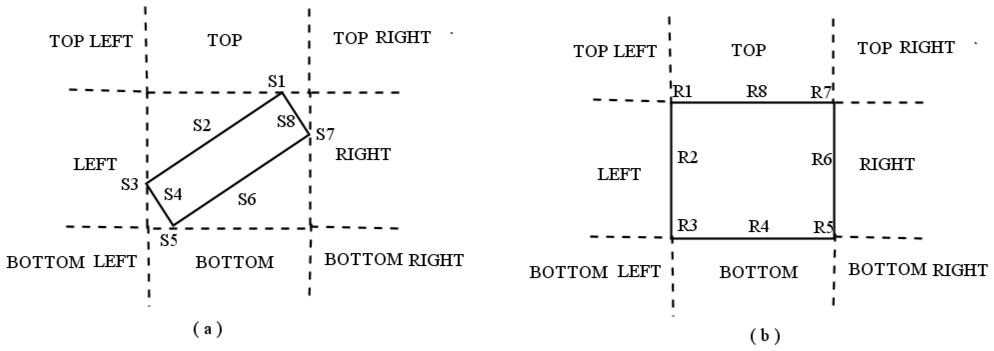
\includegraphics[scale=0.25]{EGSR-relations.png}\caption{Contact sectors and Cardinal directions of (a) an angular rectangle and (b) a normal rectangle}
\end{figure}

\section{Qualitative Motion Representation}

 To find out a best matching, a straightforward approach is to enumerate all the possible matchings. The search space is huge as there is a combinatorial number of matchings between two object sets. However, most of the matchings can be avoided by only searching through the corresponding objects in a limited area. The area of the initial object should therefore cover all the objects in the next scene that can be potentially matched to the initial object.  We use a circular region to represent such area. The circle centre is located at the centroid of the object and the radius of the circle is the maximum shift of the centroid. The radius is calculated by $V \times T$ where $V$ is the maximum velocity of the object while $T$ is the time gap. The calculation ensures the area estimation adaptable to different time gaps. We call this circle as $movement\,bounding\,circle$(MBC). 

The MBC can be divided into four quadrants to further restrict the search area. A quadrant is said to be open if all the objects in that quadrant can be considered as potential correspondence of the referred object, otherwise the quadrant is closed.  

 Given a MBC $C$, if we want to explicitly talk about the quadrants that are open, we write $C^{(i,j)}, (i,j) \in \{-, +, *\}$ wrt. the given MBC, where $(+,+)$, $(+,-)$, $(-,-)$, $(-,+)$ correspond to the top-right, top-left, bottom-left, bottom-right quadrant respectively. $(*, *)$ refers to an arbitrary quadrant. 
\begin{figure}[h!]
\centering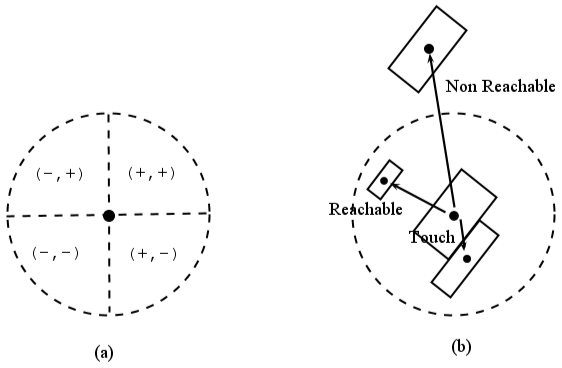
\includegraphics[scale=0.3]{quadrants.png}\caption{(a) The four quadrants of a MBC (b) Qualitative distance with respect to object A and its MBC}
\end{figure}
By estimating the movement direction of the object, we can infer the open quadrants by estimating which of the quadrants the object is most likely to be in at the next time point. The initial object will then be matched with one of the objects within the open quadrants while outside objects will not be considered.

Movement direction can be approximated by analysing the structural properties, e.g. the stability of an object. An object is stable when it is supported and remains static. When an object is not stable, there will be two possible motions: 1) free fall if it has no supports. 2) fall to the side where supports are absent. 

\cite{Ge2013} proposed four kinds of supports that can make a solid rectangle stable. We utilize these stable configurations and estimate the open quadrants accordingly. E.g. given an object supported by one edge support, if the right side support is removed, then it is likely to fall to right, thus the open quadrant is $C^{(+,-)}$
(see Figure \ref{QudrantsEstimation}). 

Movement direction of an object can also be inferred from the impact. E.g. in the angry birds scenario, we know blabla.  

\begin{figure}[h!]\label{QudrantsEstimation}
\centering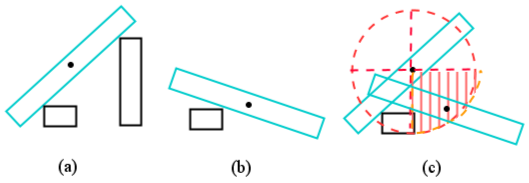
\includegraphics[scale=0.4]{QudrantsEstimation.png}\caption{(a) the object in cyan is supported via one-edge support  (b) a subsequent scene after the right support is removed (c) The estimated open quadrant (shadowed area) approximates the subsequent centroid location}
\end{figure}

Now we can distinguish the relative distance between two objects into three meaningful classes, namely touch, reachable, and non reachable. An object $O$ can touch another object $O^\prime$ by one of its contact sectors. $O^\prime$ is reachable to $O$ if $O^\prime$ is within the MBC of $O$ otherwise non reachable.



\section{Tracking by spatial reasoning}\label{trackingBySpatialReasoning}

One challenge is to find out a matching between identical objects that are close to each other, and have the similar motions.  
\begin{figure}[h!]\label{SCOExample_2}
\centering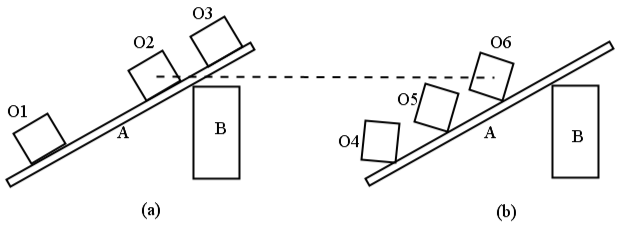
\includegraphics[scale=0.3]{SCOScenario_2.png}\caption{(a) an initial scene (b) a subsequent scene}
\end{figure}
Figure \ref{SCOExample_2}.a  shows a scene where object A and B forms a slope and there are three identical squares $O_1$, $O_2$ and $O_3$ lying on the slope. Figure \ref{}.b is a subsequent image where the three squares went down a bit. There are 6 ways to match between the squares while only $\{O_1 \sim O_4, O_2 \sim O_5, O_3 \sim O_6\}$ is possible. Without reasoning about the spatial relations between the squares, some optimization algorithms, e.g. minimizing centroid shift, will tend to match $O_2$ with $O_6$. In many cases, objects dynamics such as velocities are unavailable, thus most of state of the art tracking algorithms do not apply well because of the lack of a suitable dynamic model. 

Human can solve this case efficiently by spatial reasoning. Since we know the objects are moving at the similar velocity, the relative spatial changes among them can be subtle. Hence the spatial relations between those objects can hardly change to the opposite abruptly as they are moving. When matching, we are trying to keep the original spatial relations among the objects. 

We propose a method to deal with this in two steps, 1) identify those objects that will follow the similar motion 2) applying spatial constraints check on those objects when evaluating a match. 


We assume that the objects are likely to follow a common motion if they have the same contact relations with the same objects. We call the group of objects that are likely to share a common motion as $spatially\,\,correlated\,\,objects$ (SCO). Figure \ref{SCOExample} shows some examples of SCO in a typical angry birds scenario. 
\begin{figure}[h!]\label{SCOExample}
\centering\includegraphics[scale=0.7]{SCOScenario.png}\caption{(a) A typical angry birds scenario (b) the corresponding SCOs (highlighted by different color)}
\end{figure}
By finding groups of such objects we can then apply the spatial constraints among them when evaluating a match. 

Formally, let $R$ be a set of EGSR relations and $oppo(r), r\in R$ be the opposite set of relations of $r$. Given a group of spatially correlated objects in the initial image $O = \{o_1, o_2, ... , o_k\}$, and a set of objects in the next image $O^\prime = \{o^{\prime}_1, o^{\prime}_2, ..., o^{\prime}_k \}$ where $o_i \sim o^{\prime}_i, i \leq k$, $\exists r\in R\,\, o_i \{r\} o_j \Rightarrow \forall r^{\prime} \in oppo(r)\,\, o^{\prime}_i \{r^{\prime}\} o^{\prime}_j $ does not hold. In the slope example, a match $\{O_1 \sim O_4, O_3 \sim O_5, O_2 \sim O_6\}$ violates the constraint because $O_2 LEFT O_3$, $O_6 RIGHT O_5$ and $RIGHT \in oppo(LEFT)$  

 [list opposite set for each relation]


\section{A Method for Objects Tracking}
Let $O$ and $O^{\prime}$ be a set of objects in an initial image and a subsequent image taken at a later time, respectively. For ease of notation, we will refer to objects in $O$ as initial objects and objects in $O^{\prime}$ as new objects.

First, the method randomly assigns a unique ID to each initial object, and estimates the MBC quadrants of each object according to the object's spatial relations. The domain for each initial object is set so that it contains only the new objects that are of the same object type and within the MBC quadrants. The method then creates a preference list from the domain of each of the initial objects: the new objects in the preference list are sorted by the size of the centroid shift from the initial object in ascending order. The method matches the two sets of objects using a stable marriage algorithm with the pre-computed preference lists. The algorithm ensures each match is stable in the sense that no pair of objects would prefer each other over their matched partners. 

Then, the method finds all groups of spatially correlated objects among the initial objects and gets their corresponding objects from the match. The method then checks to see whether a spatial constraint has been violated, as mentioned in \ref{trackingBySpatialReasoning}. If there has, it resolves it accordingly.


\section{Implementation}
We implemented our method and applied it to the Angry Birds where the vision can detect the exact shapes of the objects\cite{}. The objects' visual appearance are restricted to a finite number of templates (See Fig. ).

The vision has the following limitations: 1) Damaged objects will be detected as a few separate smaller pieces. 2) Debris are not recognized so that one cannot determine whether an object, say a stone, is a real stone or just a debris from a previously destroyed stone. 3) Objects occlusion is not handled. Objects can be partially or entirely occluded by debris or other game effects e.g. prompted scores or clouds around the hit point (See Figure \ref{})

We show those problem can be dealt with effectively by the above mentioned techniques.

\subsection{Handling Fragmentation and Occlusion}

Objects fragmentation creates new objects in subsequent images and the new objects are not directly related to the initial objects. The varying number of objects from one scenario to another can introduce ambiguities making a tracking algorithm off the track. 

In angry birds, the fragmentation is mainly due to objects destruction, partially occlusion, and damage. (See Fig. ). Handling fragmentation is important. By recognizing the fragments, we are able to infer whether an object is destroyed, damaged, or occluded, which leads to a robust tracking.

We deal with the fragmentation by first recognizing potential fragments, then construct all the possible objects from the fragments, and add them to the pool of the subsequent objects for matching, and finally apply a debris recognition process for the unmatched initial objects. 

To obtain the potential fragments, we group the initial and subsequent objects according to their templates, respectively. If a group of the subsequent objects contains more objects than its initial counterpart, we treat all those subsequent objects as potential fragments.  

For all the potential fragments, we put those that can form a shape of one of the templates into a same group. The shape formed by a group of fragments is an oriented minimum bounding rectangle (OMBR) that bounds all the fragments. The fragments from one group must have the same type. We then treat the OMBR as one object in the subsequent image, which can be potentially matched with one of the initial objects. Once the OMBR is matched, all the fragments from the corresponding group are also matched. i.e. assigned with the same ID. In some rare cases, a fragment can be involved in more than one OMBRs. So we add an additional constraint: all the matched OMBRs should not have a common fragment. 

For those fragments that are not matched, we label them as debris. Destruction of an object will create a cluster of debris around the object's location. Those debris can be of any shape, e.g. circle, polygon and will diffuse until disappear after 2-4 seconds. Given an object $O$ in the initial scenario, we start the debris recognition process if there are no subsequent objects can be matched with $O$ (including the OMBRs created from the fragments). We first draw the MBC of $O$, and get the set of the subsequent objects falling in the MBC excluding those which have been matched. The set of the objects are labelled as debris of $O$ and $O$ is marked as destroyed. 

In some cases, an object can be totally occluded for a subsequence of images. To deal with this, before a matching, we cache the spatial configurations of all the initial objects. At the end of the matching, we update the cache by replacing each initial object's configuration with the matched subsequent object's so that the cache always maintains the latest configuration of each initial object. If an occluded object recurs in one subsequent image, we match the occluded object by searching through the cache for an unmatched initial object. The occlude object will be matched if it lies in the MBC of that initial object. 
  
\section{Evaluation}
We measure the accuracy of the method by the percentage of correct matches out of the total number of possible mismatches. Specifically, the mismatches 


The evaluation has been done in two phases. We first obtain the ground truth of 

\subsection{Obtaining Ground Truth}
 
 We capture a sequence of screenshots before and after a shot using the smallest time gap (50 ms). The average number of the screenshots in a typical sequence is around 200, i.e. the time gap from the beginning to the end screenshot is about 10 seconds. 

 We apply our method on the whole sequence so that the method will keep tracking the objects through all of the screenshots, from the first until the last. The match between the initial objects in the first screenshot and the subsequent objects in the last screenshot will be saved as ground truth for later evaluation.

To automate the evaluation process, we run an angry birds agent that always aims at a random pig on the first 21 Poached Eggs Levels \cite{}. The agent starts to capture screenshots 3 seconds after a shot is made, and stops after another 10 seconds. In each level, the agent records the screenshots of at most two shots. In the end, we got around 40 samples. Then we run our method on 10 out of the 40 samples, which are randomly picked. We evaluate the matchings by manually labelling the initial objects and their correspondence in the end screenshot.  



\subsection{Experimental Results}

We evaluate our method on the 40 previously collected samples with varying time gaps, namely 200 ms (the maximum delay in getting screenshot from the server of angry birds AI competition), and 300 ms (the time taken by taking a screenshot plus the vision segmentation). When evaluating with the time gap of 200 ms or 300 ms, The method will pick up one of every 200/50 = 4 or 300/50 = 6 screenshots from the original sequence, and obtain the matching accuracy by compare against the ground truth.  





\subsection{Conclusion}










\begin{algorithm}[!]
\caption{The Object Tracking Algorithm}\label{algo}
\begin{algorithmic}[1]
\Procedure {MatchObjects}{$objs$}
\State $iniobjs$ //initial objects
\State $solution \leftarrow \{iniobjs, \{\}\}$
\State $domain \leftarrow \{\}$// A map stores each initial object and a list of possible correspondence 
\State $domain \leftarrow$ MotionEstimation($objs$) 
\State CalculatePreference($iniobjs$, $domain$) //Calculate the preference list of $iniobjs$
\State $freeobjs \leftarrow iniobjs$
\While{$freeobjs$ is not empty}
\State $iniobj \leftarrow freeobjs.pop()$
\State get a next preferred $obj$ from $iniobj$'s preference list  
\If {$obj$ is not assigned yet}
  \State match($iniobj$, $obj$)
  \Else{$obj$ has been assigned to $iniobj^{\prime}$}
  \If{$obj$ prefers $iniobj$ to $iniobj^{\prime}$}
  \State match($iniobj$, $obj$), add $iniobj^{\prime}$ to $freeobjs$
\EndIf 
\EndIf
\EndWhile
\State $cobjsList \leftarrow$ GetSCO($objs$)// get spatially correlated objects
\State SPC($solution$) //Spatial Constraints Check
\State $iniobjs \leftarrow objs$
\EndProcedure

\Procedure{GetSCO}{$objs$}
\State $cobjsList \leftarrow \{\}$
\For {$obj \in objs$}
\State $cobjs \leftarrow objs$ 
\State $tobjs \leftarrow$ a set of the objects that touch $obj$
\For {$tobj \in tobjs$}
\State $ttobjs \leftarrow$ a set of the objects excluding $obj$ that touch $tobj$ via the same contact relation.
\State $cobjs \leftarrow cobjs \cap ttobjs$
\EndFor
\State $cobjsList \leftarrow cobjsList \cup cobjs$
\EndFor
\Return $cobjsList$
\EndProcedure
\Procedure{MotionEsimation}{$objs$}
\For {$obj \in objs$}
\State $domain \leftarrow domain \cup \{obj, \{\}\}$
\State $pobjs \leftarrow \{\}$
\State compute the MBC of $obj$
\State analyse the stability of $obj$ according the rules specified in \ref{} and locate the corresponding quadrants.
\State Remove the objects which are of different type, and add the remaining objects in the quadrants to $pobjs$. 
\State $domain \leftarrow domain \cup \{obj, \{pobjs\}\}$
\EndFor
\Return $domain$
\EndProcedure
\Procedure{Match}{$iniobj$, $obj$}
\State $obj.id \leftarrow iniobj.id$, $solution \leftarrow \{iniobj, obj\}$
\EndProcedure
\Procedure{SPC}{$solution$}
\For {$cobjs \in cobjsList$}
\State for each object in $cobjs$, get its matched $obj$ from $solution$
\State Check whether the spatial constraints \ref{} are violated. If violated, re-assign the objects until violation is resolved  
\EndFor
\EndProcedure
\end{algorithmic}
\end{algorithm}
 \end{document}